\documentclass[a4paper]{article}
\usepackage[pdftex]{graphicx}
\usepackage[utf8]{inputenc}
\usepackage{enumerate}
\usepackage{href-ul}
\hypersetup{
	colorlinks=true,
	linkcolor=blue,
	urlcolor=blue}
\usepackage{siunitx}
\sisetup{locale=DE} 
\usepackage{icomma}
\usepackage{amssymb}
\usepackage{geometry}
\geometry{a4paper, top=15mm, left=15mm, right=15mm, bottom=15mm,
	headsep=10mm, footskip=12mm}
\usepackage{tikz}
\usetikzlibrary{positioning}

\begin{document}

\begin{enumerate}[1.]
{\bf \item Elektrische Grundgrößen}
\begin{center}
	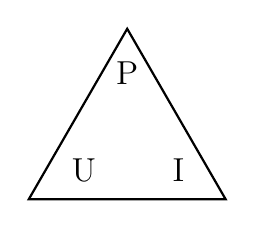
\begin{tikzpicture}[scale=1]
	% Dreieck mit Seitenlänge 2.5 cm
	\coordinate (U) at (0,0);
	\coordinate (I) at (2.5,0);
	\coordinate (P) at (1.25, {2.5*sqrt(3)/2});
	
	% Linien zeichnen
	\draw[thick] (U) -- (I) -- (P) -- cycle;
	
	% Beschriftung innerhalb
	\node[above=0.1cm of U, xshift=0.7cm] {\large U};
	\node[above=0.1cm of I, xshift=-0.6cm] {\large I};
	\node[below=0.3cm of P] {\large P};
\end{tikzpicture}
\hspace{3 cm}
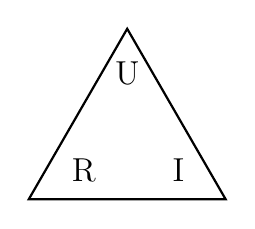
\begin{tikzpicture}[scale=1]
	% Dreieck mit Seitenlänge 2.5 cm
	\coordinate (R) at (0,0);
	\coordinate (I) at (2.5,0);
	\coordinate (U) at (1.25, {2.5*sqrt(3)/2});
	
	% Linien zeichnen
	\draw[thick] (R) -- (I) -- (U) -- cycle;
	
	% Beschriftung innerhalb
	\node[above=0.1cm of R, xshift=0.7cm] {\large R};
	\node[above=0.1cm of I, xshift=-0.6cm] {\large I};
	\node[below=0.3cm of U] {\large U};
\end{tikzpicture}
\end{center}

\renewcommand{\arraystretch}{2}
\begin{tabular}{|p{0.5 cm}|p{1.7 cm}|p{1.7 cm}|p{1.7 cm}|p{1.7 cm}|p{1.7 cm}|p{1.7 cm}|p{1.7 cm}|p{1.7 cm}|}
	\hline
	 & Wasser\-kocher & LED & Elektroauto & Notebook & Router & Wasser\-kraftwerk & Energie\-sparlampe & Gewitter\-Blitz\\
	 \hline
	 U & 230 V  &           &       &  20 V  & 12 V        &              & 230 V & $\SI{1e8}{\volt}$\\
	 \hline
	 I &        & 20 mA       & 123 A & 3,25 A &             &              &       & $\SI{1e5}{\ampere}$\\
	 \hline
	 P & 1200 W &           & 80 kW &        &             & 20 MW        &  7 W  & \\
	 \hline
	 R &       &$\SI{125}{\ohm}$&       &        & $\SI{3,6}{\ohm}$& $\SI{0,6}{\kilo\ohm}$&       & \\
	 \hline
\end{tabular}

{\bf \item Transformator}

\renewcommand{\arraystretch}{2}
\begin{tabular}{|p{2 cm}|p{2 cm}|p{2 cm}|p{2 cm}|p{2 cm}|p{2 cm}|p{2 cm}|}
	\hline
	         & $U_p$ & $U_s$ & $N_p$ & $N_s$ & $I_p$  & $I_s$ \\
	\hline
	Netzteil & 230 V & 12 V  & 500   &       & 0,12 A & \\
	\hline
	Schweißgerät &   & 50 V  & 610   & 80    &        & 160 A \\
	\hline 
Hochspan\-nungstrafo &  & 380 kV & 12  &       & 500 A  & 20 A \\
    \hline
\end{tabular}

{\bf \item Stromstärke und Ladung}
\begin{enumerate}[a)]
	\item Ein Ladegerät liefert den Strom $I=\SI{2}{\ampere}$. wie lange dauert es, bis ein Akku mit einer Kapazität von $\SI{4000}{\milli\ampere\hour}$ damit vollständig geladen ist?
	\item Derselbe Akku versorgt ein Smartphone 48 Stunden mit Energie. Wie groß ist die durchschnittliche Stromaufnahme?
	\item Ein Gold-Cap (kleiner Akkumulator) speist eine Fahrrad-Rücklicht-LED 12 Minuten lang mit Strom der Stärke 20 mA. Wie groß ist die Kapazität in (mAh) ?
	\item Ein Klein-Elektrofahrzeug kann eine Stunde mit 6,0 kW Leistung fahren. Wie groß ist die Akkukapazität in Ah, wenn die Betriebsspannung 60 V beträgt? 
\end{enumerate}


\end{enumerate} 
\fbox{
	\begin{minipage}{0.5\textwidth}
		Zur Lösung bitte \href{https://www.okuyakl.de/phys/p8puiL085/ll085.pdf}{hier klicken} oder den QR-Code scannen.\\
	Weitere Arbeitsblätter gibt es unter 
	
	\href{https://www.okuyakl.de}{www.okuyakl.de}
	\end{minipage}
	\hfill
	\begin{minipage}{0.4\textwidth}
		\includegraphics[width=1.5 cm]{../../viecher/zwe03}
		\includegraphics[width=3 cm]{qr085}
		\includegraphics[width=2 cm]{../../viecher/afanticon1}
		
	\end{minipage}}
\end{document}